\documentclass[a4paper]{article}
\usepackage[utf8]{inputenc}
\usepackage[french]{babel}
\usepackage[T1]{fontenc}
\usepackage{lmodern}
\usepackage[left=2cm,right=2cm,top=2cm,bottom=2cm]{geometry}
\usepackage{graphicx}
\usepackage{subfigure}
\usepackage{enumitem}
\usepackage{stmaryrd}
\usepackage{amsmath}
\usepackage{amssymb}
\usepackage{amsthm}
\usepackage{multicol}
\usepackage[hidelinks]{hyperref}
\usepackage{color}
\usepackage{pdfpages}
\usepackage{ebproof}
\usepackage{minted}
\usepackage{manfnt}
\usepackage[bottom]{footmisc}

\usemintedstyle{tango}

\DeclareUnicodeCharacter{393}{$\Gamma$}
\DeclareUnicodeCharacter{22A2}{$\vdash$}
\DeclareUnicodeCharacter{2203}{$\exists$}
\DeclareUnicodeCharacter{2200}{$\forall$}

\makeatletter
\AtBeginEnvironment{minted}{\dontdofcolorbox}
\def\dontdofcolorbox{\renewcommand\fcolorbox[4][]{##4}}
\makeatother

\newcommand{\N}{\ensuremath{\mathbb{N}}}
\newcommand{\Z}{\ensuremath{\mathbb{Z}}}
\newcommand{\Q}{\ensuremath{\mathbb{Q}}}
\newcommand{\znz}{\ensuremath{\mathbb{Z} / n \mathbb{Z}}}
\newcommand{\G}{\Gamma}
\DeclareMathOperator{\fv}{\mathrm{fv}}
\DeclareMathOperator{\bv}{\mathrm{bv}}
\DeclareMathOperator{\Succ}{\mathrm{Succ}}
\renewcommand{\epsilon}{\varepsilon}
\renewcommand{\leq}{\leqslant}
\renewcommand{\geq}{\geqslant}
\newcommand{\defi}{\overset{\text{def}}{=}}
\newcommand{\PA}{\mathsf{PA}}
\newcommand{\HA}{\mathsf{HA}}
\newcommand{\ZF}{\mathsf{ZF}}
\newcommand{\NJ}{\mathsf{NJ}_1}
\newcommand{\NK}{\mathsf{NK}_1}

\newcommand{\fonc}[5]{#1 : 
\left|
\begin{array}{ccc}
#2 & \longrightarrow & #3 \\
#4 & \longmapsto & #5
\end{array}
\right.
}

\newtheorem{theorem}{Théorème}[section]
\newtheorem{coro}{Corollaire}[theorem]
\newtheorem{lemma}[theorem]{Lemme}
\newtheorem{prop}[theorem]{Proposition}
\theoremstyle{remark}
\newtheorem*{rmq}{Remarque}
\theoremstyle{remark}
\newtheorem*{notation}{Notation}
\theoremstyle{remark}
\newtheorem{exemple}{Exemple}[section]
\theoremstyle{definition}
\newtheorem{df}[theorem]{Définition}
\theoremstyle{definition}
\newtheorem{algo}[theorem]{Algorithme}
\theoremstyle{definition}
\newtheorem{pb}[theorem]{Problème}

\usepackage{titlesec}
\titleformat*{\section}{\bf\Large\sffamily}
\titleformat*{\subsection}{\bf\large\sffamily}
\titleformat*{\subsubsection}{\bf\sffamily}

\title{Extensions d'un cours de logique du premier ordre certifié en Coq}
\author{Samuel Ben Hamou}
\date{\today}

\begin{document}

\includegraphics[scale=0.45]{logo_ens.png} \hfill 
\includegraphics[scale=0.1]{logo-irif.png}
\begin{center}
    \vspace*{1em}
    {\LARGE Rapport de stage} \\ \vspace{1em}
    {\huge Extensions d'un cours de logique du premier ordre certifié en Coq} \\ \vspace{2em}
    
    {\Large Stage effectué du 1 juin au 17 juillet 2020} \\ \vspace{3em}
    
    {\Large Samuel Ben Hamou} \\ \smallskip
    {\large \'Ecole Normale Supérieure Paris-Saclay} \\ 
    {\large 1ère année, Département Informatique} \\ \vspace{2em}
    
    {\Large Sous la supervision de Pierre Letouzey} \\ \smallskip
    {\large IRIF, INRIA et CNRS} \vspace{2em}
\end{center}


\begin{abstract}
Ce stage de recherche de fin de licence avait pour but de proposer des extensions à un encodage en Coq déjà existant de la déduction naturelle. Le dépôt du projet se trouve dans la branche \og Stage \fg{} à l'adresse suivante : \url{https://gitlab.math.univ-paris-diderot.fr/letouzey/natded}.

Dans un premier temps, il a fallu se familiariser avec les outils du stage : à la fois la manipulation de Git mais aussi l'encodage parfois étonnant des notions classiques de la logique (formules closes, variables liées, modèles, etc.). Un fois ce travail de défrichage effectué, nous avons pu enrichir le codage existant en suivant trois axes principaux, qui correspondent aux trois sections principales de ce rapport :
\begin{itemize}
\item l'arithmétique de \textsc{Peano}, qui avait déjà été encodée mais où tout restait à faire du point de vue des exemples et de la maniabilité des preuves,
\item la théorie des ensembles $\ZF$, où il s'est agit non seulement d'encoder les axiomes et de faire quelques preuves exemples, mais aussi de proposer une construction de $\N$,
\item le $\lambda$-calcul enfin, où nous avons pu établir la correspondance de \textsc{Curry-Howard} pour des logiques de plus en plus expressives.
\end{itemize}
\end{abstract}

\renewcommand{\contentsname}{\centerline{Table des matières} \vspace*{-2em}}
\tableofcontents

\newpage

\section{Introduction}

\subsection{Contexte pratique du stage}

Ce stage a été effectué sous la direction de Pierre Letouzey, maître de conférence à l'Université Paris-Diderot, et membre du groupe $\pi r^2$ de l'IRIF. Compte tenu du contexte sanitaire, la majeur partie des échange a eu lieu par visio-conférence et par mail, à un rythme assez soutenu. J'ai cependant pu me rendre physiquement à l'IRIF afin de discuter dans la vraie vie avec avec mon maître de stage.

Malgré les échanges de mails réguliers, le travail à distance a probablement été le plus gros inconvénient de ce stage : dans la mesure où je travaillais sur un codage créé par Pierre Letouzey, qui n'a pas écrit de manuel d'explication pour justifier ou expliquer ses choix d'implémentation (ce qui se conçoit parfaitement étant donné l'usage qu'il avait prévu de faire de son travail, qui n'était censé être utilisé que pour illustrer le cours de logique qu'il donne en M1), j'ai dans eu grandement besoin d'explications pour me lancer dans le travail, et il eût probablement été plus aisé d'avoir ce genre de discussions informelles si nous avions pu travailler dans deux bureaux adjacents.

Il n'en demeure pas moins que le stage a pu se dérouler sans trop d'embûches, et sans problèmes matériels majeurs. Par ailleurs, le travail à distance présente l'avantage non négligeable de permettre à chacun de travailler aux horaires qui lui conviennent le mieux, fût-ce tard le soir (ou bien tôt le matin selon la façon dont on voit les choses).

\subsection{Motivations}

Le but du stage a été d'enrichir l'encodage de \verb+NatDed+ déjà existant, tout en gardant en tête la vocation pédagogique du projet, puisqu'il s'agit d'illustrer un cours de logique de M1 \cite{poly}.

\verb+NatDed+ étant à l'origine assez rustique, il était pédagogiquement intéressant de le rendre plus \textit{user-friendly}, mais aussi d'ajouter un certain nombre d'exemples et d'applications (la théorie $\ZF$ par exemple), qui manquaient au projet initial.

Par la suite, il a été à propos d'ajouter d'autres aspects de la logique à cet encodage, tels que le $\lambda$-calcul, la théorie des ensembles et éventuellement la logique intuitionniste (en particulier les modèles de \textsc{Kripke}), qui sont tous des point abordés dans le cours donné par Pierre Letouzey. En effet, le $\lambda$-calcul est un élément essentiel de la construction des assistants de preuve tels que Coq.

\subsection{Encodage existant et état de l'art}

L'encodage \verb+NatDed+ existant déjà avant le stage. \`A ce moment là, il contenait déjà un système de déduction naturelle avec des séquents, ainsi qu'un grand nombre de lemmes et résultats utiles, y compris sur la méta-théorie. Deux méthodes sont possibles pour établir une preuve dans cette encodage : une méthode constructive, reposant sur le prédicat \verb+Pr+ dont la définition est donnée en annexe \ref{pr}, qui permet de construire une preuve pas à pas, mais n'est pas forcément pratique à utiliser pour démontrer des résultats méta-théoriques. L'autre méthode, \verb+Valid+, permet de vérifier qu'une dérivation est bien formée (cela implique donc de fournir directement une dérivation complète, ce qui alourdi considérablement le style des preuves). Le choix qui a été fait pour stage est d'utiliser \verb+Pr+ systématiquement.

En ce qui concerne la façon d'encoder les formules de la logique du premier ordre, Pierre Letouzey avait choisi un système \emph{locally nameless}, i.e. où les variables liées sont représentées par des indices de \textsc{de Bruijn} et les variables libres par un nom du type \verb+FVar string+ (par exemple $x$ s'écrira \verb+FVar "x"+). En parallèle de cette convention, une équivalence avec un système reposant totalement sur des variables nommées était proposée, mais quoiqu'elle eût peut se révéler fort utile, cette équivalence n'a guère été utilisée pendant le stage.
\medskip

A priori, il s'agit du premier codage Coq de la déduction naturelle qui allie les trois aspects suivants :
\begin{itemize}
\item \emph{Calcul} : l'ensemble du système n'est pas purement syntaxique, puisqu'il tire également partie de la capacité de Coq à effectuer un certain nombre de calculs à la place de l'utilisateur. Par exemple, les substitutions sont entièrement gérées par une fonction \verb+bsubst+.
\item \emph{Méta-théorie} assez poussée, dans la mesure où un théorème de complétude a pu être démontré.
\item \emph{Pédagogie} : avec un peu de patience -- et, je l'espère, en s'aidant du travail effectué pendant le stage -- on peut utiliser ce codage pour illustrer un cours sur la théorie de la démonstration, ou bien justifier que l'on peut admettre un certain nombre de résultats longs à démontrer en exhibant une preuve (plus ou moins lisible à l'\oe il nu) dans ce système.
\end{itemize}

\subsection{Mise en place de l'environnement de travail}

Avant de se lancer dans le stage à proprement parler, il a fallu consacrer une petite semaine à l'acquisition de réflexes de travail, à la fois sur le support (GitLab) et sur l'encodage lui-même.

\subsubsection{Dépôt Git}

La première journée du stage a été passée à appréhender un outil nouveau pour manipuler de gros projets de code : GitLab. \'A ce titre, et pour me fixer les idées, j'ai rédigé la cheatsheet présentée en \ref{gitsheet}.

L'usage de Git a été d'un grand recours, notamment lorsque nous voulions discuter d'un morceau de preuve en visio-conférence, car chacun pouvait travailler et mettre à jour le dépôt de son côté, la fusion se faisant ensuite aisément grâce à la commande \verb+git pull+.

\subsubsection{Premières preuves}

Afin de me faire la main sur un encodage déjà très évolué, j'ai tenté de démontrer les petits résultats classiques suivants :
\begin{itemize}
\item $\vdash (\phi_1 \wedge \phi_2) \Rightarrow (\phi_1 \vee \phi_2)$,
\item $\vdash (\phi_1 \Rightarrow \phi_2 \Rightarrow \phi_3) \Leftrightarrow (\phi_1 \wedge \phi_2 \Rightarrow \phi_3)$,
\item $\vdash \phi \vee \neg \phi$.
\end{itemize}
Pour ce dernier point, il a été utile d'établir l'admissibilité des règles suivantes : \[ \begin{prooftree}
\hypo{\Gamma \vdash \neg \neg \phi}
\infer1[RAA]{\Gamma \vdash \phi}
\end{prooftree} \qquad \begin{prooftree}
\hypo{\Gamma \vdash \neg (\neg \phi_1 \wedge \phi_2)}
\infer1[Morgan]{\Gamma \vdash \phi_1 \vee \neg \phi_2}
\end{prooftree} \] puisque la règle de l'absurde présente dans l'encodage initial était \begin{prooftree*}
\hypo{\neg \phi, \Gamma \vdash \bot}
\infer1[absu]{\Gamma \vdash \phi}
\end{prooftree*}
\'Evidemment, les règles RAA et absu sont équivalentes, mais la forme RAA était plus commode pour montrer le tiers-exclu.

\`A titre d'illustration, voici l'énoncé de ces petits résultats tels que démontré dans le projet. On donne également la démonstration du premier, afin d'avoir une idée de ce à quoi ressemble une preuve en déduction naturelle dans cet encodage.

\begin{minted}{coq}
Lemma ex1 f1 f2 : Provable Intuiti ([] ⊢ (f1 /\ f2) -> (f1 \/ f2)).
Proof.
  apply Provable_alt.
  apply R_Imp_i.
  apply R_Or_i1.
  apply R_And_e1 with (B := f2).
  apply R_Ax.
  apply in_eq.
Qed.

Lemma ex2 f1 f2 f3 : Provable Intuiti ([] ⊢ (f1 -> f2 -> f3) <-> (f1 /\ f2 -> f3)).

Lemma RAA f1 Γ : Pr Classic (Γ ⊢ ~~f1) -> Pr Classic (Γ ⊢ f1).

Lemma DeMorgan f1 f2 Γ : Pr Classic (Γ ⊢ ~(~f1 /\ f2)) -> Pr Classic (Γ ⊢ ~~(f1 \/ ~f2)).

Lemma ExcludedMiddle f1 : Provable Classic ([] ⊢ f1 \/ ~f1).
\end{minted}

\noindent \begin{minipage}[t]{0.05\linewidth}
\dbend
\end{minipage} \begin{minipage}[c]{0.95\linewidth}
Les symboles \verb+->+, \verb+/\+, \verb+\/+ et \verb+~+ utilisés à l'intérieur des séquents n'ont \emph{rien à voir} avec les opérateurs Coq du même nom : il s'agit d'une surcharge de notation pour rendre les preuves plus lisibles.
\end{minipage}

\section{Arithmétique de {\sc Peano}}

\subsection{Constats de départ}

L'encodage de $\PA$ contenait déjà les axiomes ainsi que quelques éléments méta-théoriques. En outre, un prédicat \verb+IsTheorem+ définit comme suit :
\begin{minted}{coq}
Definition IsTheorem th T :=
  Wf th T /\
  exists axs,
    Forall th.(IsAxiom) axs /\
    Pr logic (axs ⊢ T).
\end{minted}
dans le fichier \verb+Theories.v+ permet d'énoncer des théorèmes en prenant en compte le fait que les séquents à dériver respectent bien la signature de la théorie, et que les axiomes choisis sont licites.

Mon premier travail a été de mettre cet encodage à l'épreuve, afin de pouvoir ensuite déterminer les points à améliorer, et comparer la longueur des preuves avec et sans tactiques adjuvantes. Le but, bien entendu, était d'écrire les tactiques les plus générales possible, et ce pari a été plutôt réussi puisque certaines d'entre elles ont pu être réutilisées dans \verb+ZF.v+ par la suite. \`A cet effet, les résultats suivants ont été démontrés :
\begin{minted}{coq}
Lemma ZeroRight : IsTheorem Intuiti PeanoTheory (∀ (#0 = #0 + Zero)).

Lemma SuccRight : IsTheorem Intuiti PeanoTheory (∀∀ (Succ(#1 + #0) = #1 + Succ(#0))).

Lemma Comm :
  IsTheorem Intuiti PeanoTheory
            ((∀ #0 = #0 + Zero) -> (∀∀ Succ(#1 + #0) = #1 + Succ(#0)) ->
               (∀∀ #0 + #1 = #1 + #0)).

Lemma Commutativity : IsTheorem Intuiti PeanoTheory (∀∀ #0 + #1 = #1 + #0).
\end{minted}
Le but initial a été de démontrer la commutativité de la loi $+$ dans le cadre de $\PA$, cependant, quelques lemmes intermédiaires furent nécessaires. L'existence d'un lemme \verb+Comm+ et d'un autre lemme \verb+Commutativity+ illustre la première pierre d'achoppement de l'encodage existant des théories : l'impossibilité d'utiliser des lemmes auxiliaires dans le corps d'une preuve. La solution proposée dans ce problème est détaillée en section \ref{sol}.

Par ailleurs, les débuts de preuve avaient tendance à être particulièrement inintéressants et répétitifs : passer la liste des axiomes de \textsc{Peano} en argument à la quantification existentielle\footnote{Avec toutefois un petit problème lorsqu'il s'agissait de raisonner par récurrence, puisque le schéma d'axiome de récurrence engendre une infinité d'axiomes, ce que Coq a beaucoup de mal à gérer.}, justifier que la formule que l'on souhaite montrer respecte bien la signature de $\PA$, initier un raisonnement par récurrence avec la bonne instance du schéma d'axiome de récurrence si nécessaire. Tous ces éléments rendaient les preuves lourdes et paraissaient pourtant hautement automatisables.

Quelques propriétés utiles étaient par ailleurs sans cesse utilisées. Si la transitivité et la symétrie de l'égalité font partie de toute théorie égalitaire qui se respecte, le besoin de règles de dérivation telles que \begin{prooftree*}
\hypo{\Gamma \vdash u = v}
\infer1[sym]{\Gamma \vdash v = u}
\end{prooftree*} se fait cruellement ressentir. En l'état, l'utilisation de l'axiome de symétrie de l'égalité nécessitait d'avoir recours à la tactique \verb+assert+ pour rajouter un jugement précisant que le séquent $\PA \vdash \forall x, \forall y \cdot x = y \Rightarrow y = x$ est dérivable, puis d'utiliser les règles d'élimination adéquates. Il en va de même pour les axiomes du type $\forall x, \forall y \cdot x = y \Rightarrow \Succ (x) = \Succ (y)$.

Enfin, certaines tactiques et règles définies dans l'encodage de \verb+NatDed+ étaient passablement pénibles à utiliser. Entre autres, on peut citer \verb+R_All_i+, la règle d'introduction du quantificateur universel, qui engendrait un grand nombre de buts ennuyants à démontrer. On peut également mentionner tous les résultats faisant intervenir des ensembles finis, par exemple le lemme d'affaiblissement, car la représentation de ces ensembles en Coq est surprenante et se prête fort mal à des tactiques de simplification usuelles telles que \verb+cbn+ ou \verb+omega+.

\subsection{Définition de nouvelles tactiques}

Afin de régler les susmentionnés problèmes, j'ai mis au point un certain nombre de tactiques censées rendre les preuves plus courtes et plus lisibles, en somme plus proches des preuves que l'ont ferait sur papier. L'objectif ultime étant que l'on puisse facilement voir émerger l'arbre de dérivation du séquent que l'on est en train de démontrer. Afin de constater l'apport de ces nouvelles tactiques, une mise en regard des preuves du lemme \verb+ZeroRight+ avant et après simplifications et proposée en annexe \ref{beforeafter_zeroright}.

\subsubsection{Pour les débuts de preuve}

Dans l'objectif d'alléger les débuts de preuve, j'ai mis en place deux tactiques distinctes.
\smallskip

La première, \verb+thm+, permet de traiter à peu de frais le but \verb+Wf th T+, qui permet juste de vérifier que la formule à démontrer respecte la signature de la théorie $T$. Sa mise en place a été relativement aisée car la preuve du but qu'elle entend éliminer est toujours la même, indépendamment du théorème à démontrer ou de la théorie considérée. Il a donc suffit de copier-coller la preuve donnée dans \verb+ZeroRight+ (par exemple) pour obtenir cette tactique qui a fonctionné quasiment du premier coup. \'Evidemment, le stage avançant, la tactique a été enrichie par d'autres tactiques permettant notamment de calculer plus efficacement sur les listes, etc.
\smallskip

La seconde tactique élaborée n'est pas à utiliser systématiquement. Elle permet, à partir du but fourni par la tactique \verb+thm+ de trouver la bonne instance $A$ du schéma d'axiome de récurrence et d'instancier ensuite la quantification existentielle par \verb$(induction_schema A) :: axioms_list$.

Concrètement, cette tactique s'appuie sur une tactique auxiliaire \verb+parse+ qui prend en argument une formule $\phi$ contenant au moins une quantification universelle sous la forme non-restrictive \[ \phi_1 \Rightarrow \cdots \Rightarrow \forall x \cdot \phi_n \] avec éventuellement $n = 1$, et qui retourne $\phi_n$. Une fois la formule $\phi_n$ identifiée, \verb+rec+ l'utilise pour instancier le schéma d'axiome de récurrence et initie la preuve, de sorte que l'utilise se retrouve avec deux buts, qui correspondent à l'initialisation et à l'hérédité de la preuve par récurrence. Pour ce faire, j'ai eu besoin de prouver deux lemmes auxiliaires qui permettent essentiellement de montrer que l'instance du schéma d'axiome de récurrence choisie est bien licite, et qui proposent une forme plus facilement manipulable du principe de récurrence.

Il est à noter que, en allant chercher le premier quantificateur universel qu'elle trouve dans la formule, \verb+parse+ ne restreint pas la généralité de la tactique \verb+rec+. En effet, les quantificateurs universels commutent évidemment, et si un le théorème $\phi$ à démontrer contient un quantificateur existentiel, on peut toujours éliminer les quantificateurs qui le précèdent (avec les règles \verb+R_All_i+ et \verb+R_Ex_i+) afin d'appliquer la tactique \verb+rec+, puis les réintroduire avec \verb+R_All_e+ et \verb+R_Ex_e+. Cela revient essentiellement à utiliser les tactiques \verb+intro+ et \verb+exists+ avant de lancer un \verb+induction+ en Coq, puis d'utiliser \verb+revert+ pour rétablir le théorème initial.
% TODO
% nom de l'analogue de revert pour exists

\subsubsection{Pour raccourcir certains raisonnements}

La création de tactiques permettant d'utiliser rapidement des propriétés telles que la symétrie de l'égalité ou sa compatibilité avec le prédicat $\Succ$ s'est fait en deux étapes.

Dans un premier temps, j'ai démontré les lemmes suivants :
\begin{minted}{coq}
Lemma Symmetry :
  forall logic A B Γ, BClosed A -> In ax2 Γ -> Pr logic (Γ ⊢ A = B) ->
                      Pr logic (Γ ⊢ B = A).

Lemma Transitivity :
  forall logic A B C Γ, BClosed A -> BClosed B -> In ax3 Γ ->
                        Pr logic (Γ ⊢ A = B) -> Pr logic (Γ ⊢ B = C) -> Pr logic (Γ ⊢ A = C).

Lemma Hereditarity :
  forall logic A B Γ, BClosed A -> In ax4 Γ -> Pr logic (Γ ⊢ A = B) ->
                      Pr logic (Γ ⊢ Succ A = Succ B).

Lemma AntiHereditarity :
  forall logic A B Γ, BClosed A -> In ax13 Γ -> Pr logic (Γ ⊢ Succ A = Succ B) ->
                      Pr logic (Γ ⊢ A = B).
\end{minted}

Une fois ces résultats établis, j'ai facilement pu créer les tactiques qui nous intéressaient, où il s'agissait essentiellement d'appliquer le théorème idoine et de simplifier à l'aide de tactiques de calcul spécifiques, telles que \verb+calc+ ou \verb+cbm+, qui ont été écrites par Pierre Letouzey pour faciliter la manipulation d'ensembles finis et de listes.
\smallskip

En plus de cela, j'ai aussi défini des tactiques qui permettent de gérer plus facilement la règle \verb+R_All_i+ ou d'ajouter la dérivabilité d'axiomes dans les hypothèses, pour pouvoir raisonner à rebours (i.e. de haut de bas de l'arbre de dérivation). Ces tactiques très simples ne sont finalement que des macros qui évitent d'avoir à réécrire plusieurs fois les mêmes petits bouts de preuve et de se concentrer sur l'aspect déduction naturelle plutôt que sur l'aspect Coq.

\subsubsection{Pour utiliser des lemmes auxiliaires}\label{sol}

Le principal problème posé par l'usage de lemmes auxiliaires est le fait qu'ils sont toujours de la forme \verb+IsTheorem+, alors que le corps d'une preuve fait plutôt intervenir le prédicat \verb+Pr+. La solution proposée pour palier à cela a été d'établir une espèce de modus ponens sur \verb+IsTheorem+. Plus précisément, on a démontré
\begin{minted}{coq}
Lemma ModusPonens th :
  forall A B , IsTheorem th (A -> B) -> IsTheorem th A ->
               IsTheorem th B.

\end{minted}
Grâce à ce résultat, la preuve d'un théorème $\phi$ utilisant des lemmes auxiliaires se fait en deux temps : dans un premier temps, on montre que $\phi$ est effectivement impliqué par tous les lemmes auxiliaires $\psi_1, \ldots, \psi_n$ que l'on souhaite utiliser (c'est là que repose toute la preuve), et dans un second temps, on utilise \verb+ModusPonens+ pour montrer que $\psi_1, \ldots, \psi_n$ sont bien des théorèmes eux aussi.


\section{Théorie des ensembles de {\sc Zermelo-Fraenkel}}

\subsection{Encodage des axiomes et méta-théorèmes}

\subsection{Preuves exemples}

\subsection{Construction de $\N$}

% construction de von Neumann


\section{Lien avec le $\lambda$-calcul}

\subsection{Choix de codage}

% à la Church

\subsection{Correspondance de {\sc Curry-Howard}}

Cette partie reprend les concepts et les constructions du cours de $\lambda$-calcul de Jean Goubault-Larrecq \cite{polylam}. Par ailleurs, on se placera toujours dans le cadre de la \emph{logique intuitionniste}.

Le théorème de \textsc{Curry-Howard} a ensuite été utilisé pour redémontrer le premier résultat du stage, à la savoir que le séquent $\vdash (\phi_1 \wedge \phi_2) \Rightarrow (\phi_1 \vee \phi_2)$ était dérivable. Pour ce faire il a suffit d'exhiber le $\lambda$-terme $\lambda x \cdot \iota_1 \pi_1 x$, qui est un témoin de preuve beaucoup plus aisé à manipuler qu'un arbre de dérivation complet.

\subsubsection{Logique minimale intuitionniste}

\subsubsection{Faux et opérateur $\nabla$}

% la négation se déduit facilement du faux : non A = A -> faux

\subsubsection{Conjonction : couples et projections}

\subsubsection{Disjonction : filtrage par motif et injections}


\section{Conclusion}

\bibliographystyle{plain}
%\renewcommand{\refname}{Bibliographie}
\nocite{*}
\bibliography{biblio}

\appendix
\newpage

\section{Définition de \texttt{Pr}} \label{pr}

\begin{minted}{coq}
Inductive Pr (l:logic) : sequent -> Prop :=
 | R_Ax Γ A : In A Γ -> Pr l (Γ ⊢ A)
 | R_Tr_i Γ : Pr l (Γ ⊢ True)
 | R_Fa_e Γ A : Pr l (Γ ⊢ False) ->
                  Pr l (Γ ⊢ A)
 | R_Not_i Γ A : Pr l (A::Γ ⊢ False) ->
                   Pr l (Γ ⊢ ~A)
 | R_Not_e Γ A : Pr l (Γ ⊢ A) -> Pr l (Γ ⊢ ~A) ->
                   Pr l (Γ ⊢ False)
 | R_And_i Γ A B : Pr l (Γ ⊢ A) -> Pr l (Γ ⊢ B) ->
                   Pr l (Γ ⊢ A/\B)
 | R_And_e1 Γ A B : Pr l (Γ ⊢ A/\B) ->
                    Pr l (Γ ⊢ A)
 | R_And_e2 Γ A B : Pr l (Γ ⊢ A/\B) ->
                    Pr l (Γ ⊢ B)
 | R_Or_i1 Γ A B : Pr l (Γ ⊢ A) ->
                   Pr l (Γ ⊢ A\/B)
 | R_Or_i2 Γ A B : Pr l (Γ ⊢ B) ->
                   Pr l (Γ ⊢ A\/B)
 | R_Or_e Γ A B C :
     Pr l (Γ ⊢ A\/B) -> Pr l (A::Γ ⊢ C) -> Pr l (B::Γ ⊢ C) ->
     Pr l (Γ ⊢ C)
 | R_Imp_i Γ A B : Pr l (A::Γ ⊢ B) ->
                     Pr l (Γ ⊢ A->B)
 | R_Imp_e Γ A B : Pr l (Γ ⊢ A->B) -> Pr l (Γ ⊢ A) ->
                   Pr l (Γ ⊢ B)
 | R_All_i x Γ A : ~Names.In x (fvars (Γ ⊢ A)) ->
                   Pr l (Γ ⊢ bsubst 0 (FVar x) A) ->
                   Pr l (Γ ⊢ ∀A)
 | R_All_e t Γ A : Pr l (Γ ⊢ ∀A) -> Pr l (Γ ⊢ bsubst 0 t A)
 | R_Ex_i t Γ A : Pr l (Γ ⊢ bsubst 0 t A) -> Pr l (Γ ⊢ ∃A)
 | R_Ex_e x Γ A B : ~Names.In x (fvars (A::Γ⊢B)) ->
      Pr l (Γ ⊢ ∃A) -> Pr l ((bsubst 0 (FVar x) A)::Γ ⊢ B) ->
      Pr l (Γ ⊢ B)
 | R_Absu Γ A : l=Classic -> Pr l (Not A :: Γ ⊢ False) ->
                  Pr l (Γ ⊢ A).
\end{minted}

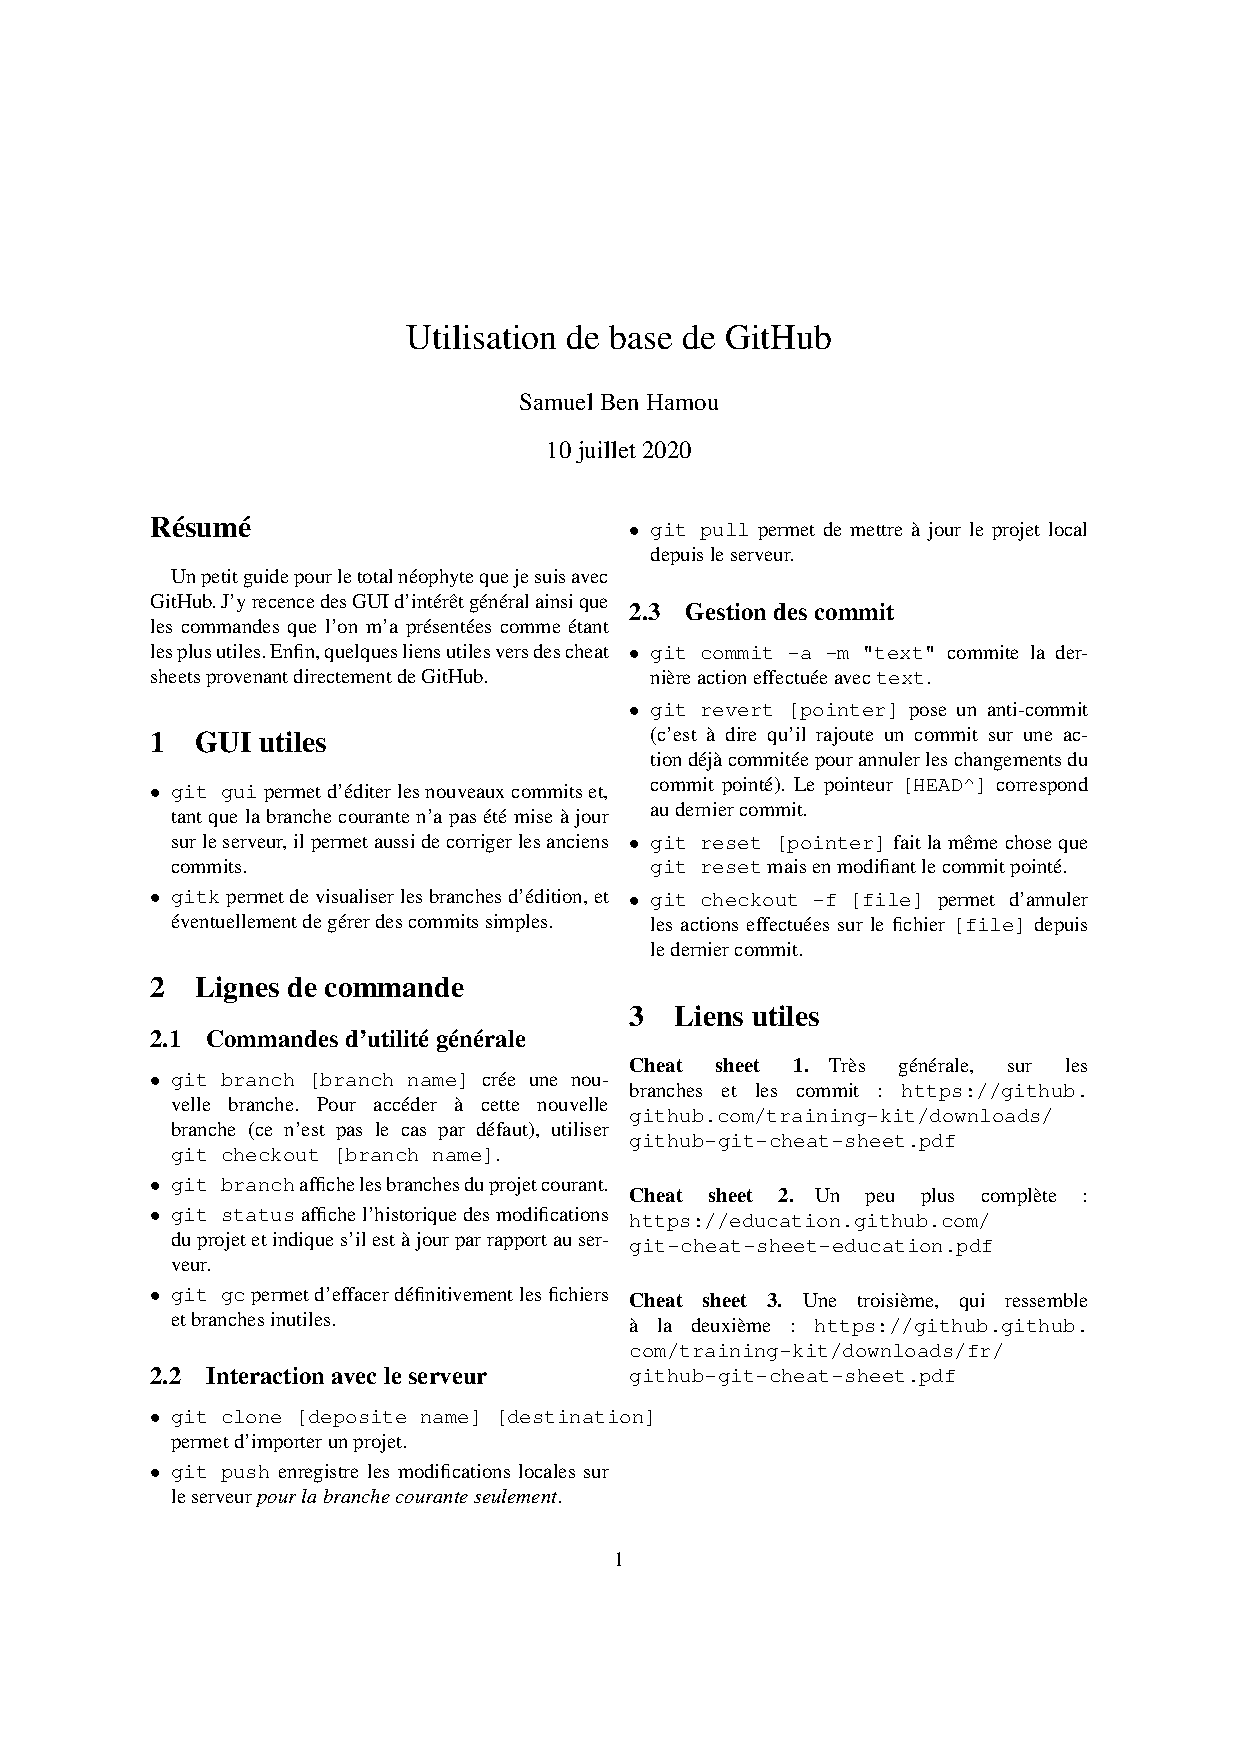
\includepdf[pages=1, nup=1x1, frame=true, scale=0.8, pagecommand=\section{Cheatsheet pour GitLab}\label{gitsheet}]{TutoGitHub.pdf}

\section{Preuve de \texttt{ZeroRight} : avant-après}\label{beforeafter_zeroright}

La preuve originelle était :
\begin{minted}{coq}
Lemma ZeroRight :
  IsTheorem Intuiti PeanoTheory
            (∀ (#0 = #0 + Zero)).
Proof.
  unfold IsTheorem.
  split.
  + unfold Wf. split; [ auto | split; auto ].
  + exists ((PeanoAx.induction_schema (#0 = #0 + Zero))::axioms_list).
    split.
    - apply Forall_forall.
      intros. destruct H.
      * simpl. unfold IsAx.
        right. exists (#0 = #0 + Zero).
        split; [ auto | split ; [ auto | auto ] ].
      * simpl. unfold IsAx. left. exact H.
    - apply R_Imp_e with
      (A := (nForall (Nat.pred (level (# 0 = # 0 + Zero)))
       ((∀ bsubst 0 Zero (# 0 = # 0 + Zero)) /\
        (∀ # 0 = # 0 + Zero -> bsubst 0 (Succ (# 0)) (# 0 = # 0 + Zero))))).
      * apply R_Ax. unfold induction_schema. apply in_eq.
      * simpl. apply R_And_i. cbn.
        change (Fun "O" []) with Zero.
        apply R_All_i with (x := "x").
        ++ compute. inversion 1.
        ++ cbn. change (Fun "O" []) with Zero.
           eapply R_Imp_e. set (hyp := (_ -> _)%form).
           assert ( sym : Pr Intuiti (hyp::axioms_list ⊢ ∀∀ (#1 = #0 -> #0 = #1))).
           { apply R_Ax. compute; intuition. }
           apply R_All_e with (t := Zero + Zero) in sym. cbn in sym.
           apply R_All_e with (t := Zero) in sym. cbn in sym. exact sym.
           -- reflexivity.
           -- reflexivity.
           -- set (hyp := (_ -> _)%form). change (Fun "O" []) with Zero.
              change (Zero + Zero = Zero) with (bsubst 0 Zero (Zero + #0 = #0)).
              apply R_All_e. reflexivity.
              apply R_Ax. compute; intuition.
       ++ cbn. change (Fun "O" []) with Zero.
          apply R_All_i with (x := "y").
          -- compute. inversion 1.
          -- cbn. change (Fun "O" []) with Zero.
             apply R_Imp_i. set (H1 := FVar _ = _). set (H2 := _ -> _).
             assert (hyp : Pr Intuiti
                              (H1 :: H2 :: axioms_list ⊢ Fun "S" [FVar "y"] =
                               Fun "S" [FVar "y" + Zero] /\
                               Fun "S" [FVar "y" + Zero] = Fun "S" [FVar "y"] + Zero)).
             { apply R_And_i.
               - assert (AX4 : Pr Intuiti (H1 :: H2 :: axioms_list ⊢ ax4)).
                 { apply R_Ax. compute; intuition. }
                 apply R_Imp_e with (A := (FVar "y" = FVar "y" + Zero)%form);
                   [ | apply R_Ax; compute; intuition ].
                 unfold ax4 in AX4. apply R_All_e with (t := FVar "y") in AX4; [ | auto ].
                 apply R_All_e with (t := FVar "y" + Zero) in AX4; [ | auto ].
                 cbn in AX4. exact AX4. 
               - apply R_Imp_e with (A := Fun "S" [FVar "y"] + Zero = Fun "S" [FVar "y" + Zero]).
                 + assert (AX2 : Pr Intuiti (H1 :: H2 :: axioms_list ⊢ ax2)).
                   { apply R_Ax. compute; intuition. }
                   unfold ax2 in AX2.
                   apply R_All_e with (t := Fun "S" [FVar "y"] + Zero) in AX2; [ | auto ].
                   apply R_All_e with (t := Fun "S" [FVar "y" + Zero]) in AX2; [ | auto ].
                   cbn in AX2. exact AX2.
                 + assert (AX10 : Pr Intuiti (H1 :: H2 :: axioms_list ⊢ ax10)).
                   { apply R_Ax. compute; intuition. }
                   unfold ax10 in AX10.
                   apply R_All_e with (t:= FVar "y") in AX10; [ | auto ].
                   apply R_All_e with (t := Zero) in AX10; [ | auto ].
                   cbn in AX10. exact AX10. }
             apply R_Imp_e with
             (A :=  Fun "S" [FVar "y"] = Fun "S" [FVar "y" + Zero] /\
                    Fun "S" [FVar "y" + Zero] = Fun "S" [FVar "y"] + Zero).
             ** assert (AX3 : Pr Intuiti (H1 :: H2 :: axioms_list ⊢ ax3)).
                { apply R_Ax. compute; intuition. }
                unfold ax3 in AX3.
                apply R_All_e with (t:= Fun "S" [FVar "y"]) in AX3; [ | auto ].
                apply R_All_e with (t := Fun "S" [FVar "y" + Zero]) in AX3; [ | auto ].
                apply R_All_e with (t := Fun "S" [FVar "y"] + Zero) in AX3; [ | auto ].
                cbn in AX3. exact AX3.
             ** exact hyp.
 Qed.    
\end{minted}
et en fin de stage, elle était devenue
\begin{minted}{coq}
Lemma ZeroRight :
  IsTheorem Intuiti PeanoTheory
            (∀ (#0 = #0 + Zero)).
Proof.
 thm.
 rec.
 + sym.
   inst_axiom ax9 [Zero].
 + app_R_All_i "y" y.
   apply R_Imp_i. set (H1 := _ = _).
   sym.
   trans (Succ (y + Zero)).
   - inst_axiom ax10 [y; Zero].
   - ahered.
     sym.
     apply R_Ax.
     apply in_eq.
Qed.
\end{minted}

\section{Syntaxe et règles de typage du $\lambda$-calcul utilisé}

La syntaxe des $\lambda$-termes est la suivante :
\begin{align*}
u, v, \ldots ::&= x, y, \ldots & \text{variables}\\
&| \; uv & \text{application} \\
&| \; \lambda x \cdot u & \text{abstraction} \\
&| \; \nabla u & \text{nabla} \\
&| \; \langle u, v \rangle & \text{couple} \\
&| \; \pi_1 u & \text{première projection} \\
&| \; \pi_2 u & \text{seconde projection} \\
&| \; \mathtt{case} \, u \, \mathtt{of} \, \iota_1 x_1 \mapsto v_1 \; | \; \iota_2 x_2 \mapsto v_2 & \text{filtrage par motif} \\
&| \; \iota_1 u & \text{première injection} \\
&| \; \iota_2 u & \text{seconde injection}
\end{align*} et celle des types est \begin{align*}
\sigma, \tau, \ldots ::&= a, b, \ldots & \text{variables de type} \\
&| \; \sigma \Rightarrow \tau & \text{type flèche} \\
&| \; \bot & \text{faux} \\
&| \; \sigma \wedge \tau & \text{type conjonction} \\
&| \; \sigma \vee \tau & \text{type disjonction}.
\end{align*}

Les règles de typage sont :
\[ \begin{array}{lcr}
\text{\begin{prooftree}
\infer0[var]{\Gamma, x : \tau \vdash x : \tau}
\end{prooftree}} &
\text{\begin{prooftree}
\hypo{\Gamma \vdash u : \sigma \Rightarrow \tau}
\hypo{\Gamma \vdash v : \sigma}
\infer2[app]{\Gamma \vdash uv : \tau}
\end{prooftree}} &
\text{\begin{prooftree}
\hypo{\Gamma, x : \sigma \vdash u : \tau}
\infer1[abs]{\Gamma \vdash \lambda x \cdot u : \sigma \Rightarrow \tau}
\end{prooftree}} \\
& & \\
&
\text{\begin{prooftree}
\hypo{\Gamma \vdash u : \bot}
\infer1[$\nabla$]{\Gamma \vdash \nabla u : \tau}
\end{prooftree}} & \\
& & \\
\text{\begin{prooftree}
\hypo{\Gamma \vdash u : \sigma \wedge \tau}
\infer1[$\pi_1$]{\Gamma \vdash \pi_1 u : \sigma}
\end{prooftree}} &
\text{\begin{prooftree}
\hypo{\Gamma \vdash u : \sigma \wedge \tau}
\infer1[$\pi_2$]{\Gamma \vdash \pi_2 u : \tau}
\end{prooftree}} &
\text{
\begin{prooftree}
\hypo{\Gamma \vdash u : \sigma}
\hypo{\Gamma \vdash v : \tau}
\infer2[paire]{\Gamma \vdash \langle u, v \rangle : \sigma \wedge \tau}
\end{prooftree}}\\
& & \\
\text{
\begin{prooftree}
\hypo{\Gamma \vdash u : \sigma}
\infer1[$\iota_1$]{\Gamma \vdash \iota_1 u : \sigma \vee \tau}
\end{prooftree}} & &
\text{
\begin{prooftree}
\hypo{\Gamma \vdash u : \tau}
\infer1[$\iota_2$]{\Gamma \vdash \iota_2 u : \sigma \vee \tau}
\end{prooftree}} \\
& & \\
&
\text{
\begin{prooftree}
\hypo{\Gamma \vdash u : \sigma \vee \tau}
\hypo{\Gamma, x_1 : \sigma \vdash v_1 : \mu}
\hypo{\Gamma, x_2 : \tau \vdash v_2 : \mu}
\infer3[pattern]{\Gamma \vdash \mathtt{case} \, u \, \mathtt{of} \, \iota_1 x_1 \mapsto v_1 \; | \; \iota_2 x_2 \mapsto v_2 : \mu}
\end{prooftree}} &
\end{array} \]

\end{document}
